\section{Insertion Sort}
\label{sec:insertion_sort}

\begin{frame}
	\frametitle{Insertion sort}
	\begin{center}
		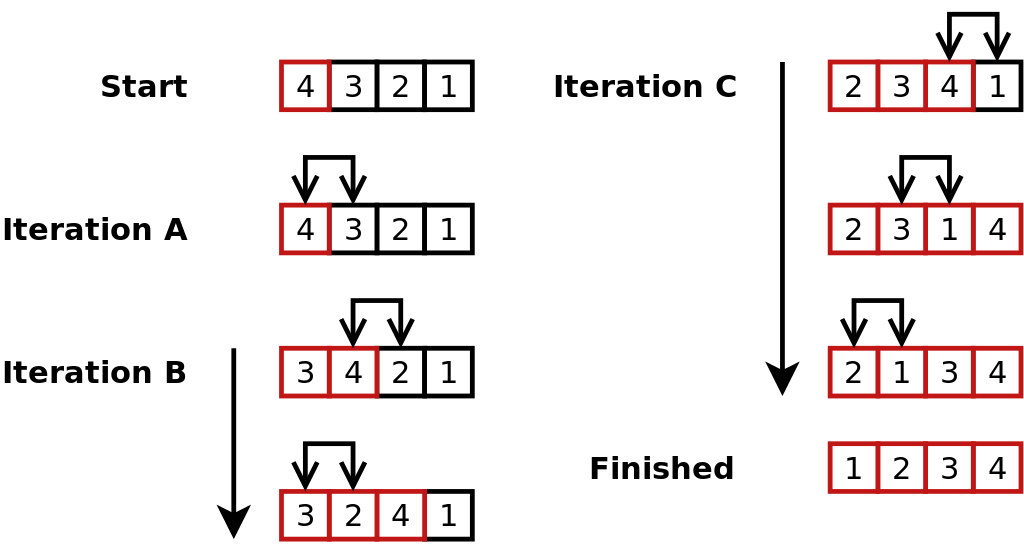
\includegraphics[width=0.8\textwidth]{figures/insertionsort.png}\\
		\hspace*{15pt}\hbox{\scriptsize Image By:\thinspace{\itshape MrDrBob}}
		% https://commons.wikimedia.org/wiki/File:Insertion-sort.svg
	\end{center}
\end{frame}

\begin{frame}
	\frametitle{Insertion Sort}
	\framesubtitle{How does that work?}
		\begin{block}{Insertion Sort}
			The main idea:
			\begin{itemize}
				\item We build the list, step by step.
					\pause
				\item We keep our intermediate result sorted.
					\pause
				\item At every step, we insert the next element into the right place.
					\pause
				\item This means we need to shift over (worst-case) $n$ elements for every element we insert...
					\pause
				\item So in total $\Theta(n^2)$ time.
			\end{itemize}
		\end{block}
\end{frame}

\begin{frame}
	\frametitle{Insertion Sort}
	\begin{algorithmic}
		\State $i \gets 1$ \Comment{The first element forms a sorted list on it's own}
		\pause
		\While{$i < \texttt{len}(l)$}
		\State $j \gets i$
		\pause
		\While{$j > 0$ and $v_{j-1} < v_{j}$}
			\State swap $v_j$ and $v_{j-1}$	
			\State $j \gets j -1$
		\EndWhile
		\pause
		\State $i \gets i+1$
		\EndWhile
	\end{algorithmic}
	\pause
	\begin{center}
	\section{Insertion Sort}
\label{sec:insertion_sort}

\begin{frame}
	\frametitle{Insertion sort}
	\begin{center}
		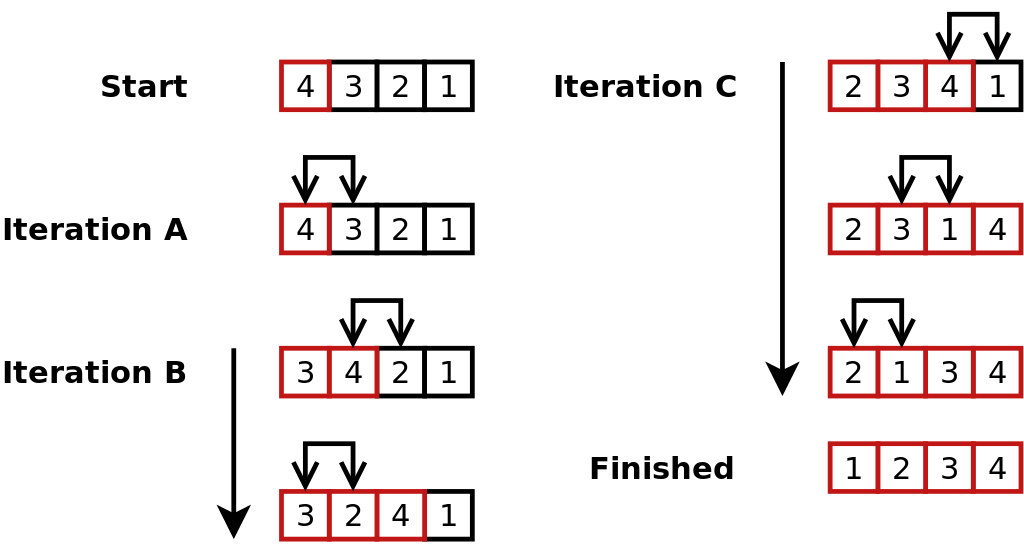
\includegraphics[width=0.8\textwidth]{figures/insertionsort.png}\\
		\hspace*{15pt}\hbox{\scriptsize Image By:\thinspace{\itshape MrDrBob}}
		% https://commons.wikimedia.org/wiki/File:Insertion-sort.svg
	\end{center}
\end{frame}

\begin{frame}
	\frametitle{Insertion Sort}
	\framesubtitle{How does that work?}
		\begin{block}{Insertion Sort}
			The main idea:
			\begin{itemize}
				\item We build the list, step by step.
					\pause
				\item We keep our intermediate result sorted.
					\pause
				\item At every step, we insert the next element into the right place.
					\pause
				\item This means we need to shift over (worst-case) $n$ elements for every element we insert...
					\pause
				\item So in total $\Theta(n^2)$ time.
			\end{itemize}
		\end{block}
\end{frame}

\begin{frame}
	\frametitle{Insertion Sort}
	\begin{algorithmic}
		\State $i \gets 1$ \Comment{The first element forms a sorted list on it's own}
		\pause
		\While{$i < \texttt{len}(l)$}
		\State $j \gets i$
		\pause
		\While{$j > 0$ and $v_{j-1} < v_{j}$}
			\State swap $v_j$ and $v_{j-1}$	
			\State $j \gets j -1$
		\EndWhile
		\pause
		\State $i \gets i+1$
		\EndWhile
	\end{algorithmic}
	\pause
	\begin{center}
	\section{Insertion Sort}
\label{sec:insertion_sort}

\begin{frame}
	\frametitle{Insertion sort}
	\begin{center}
		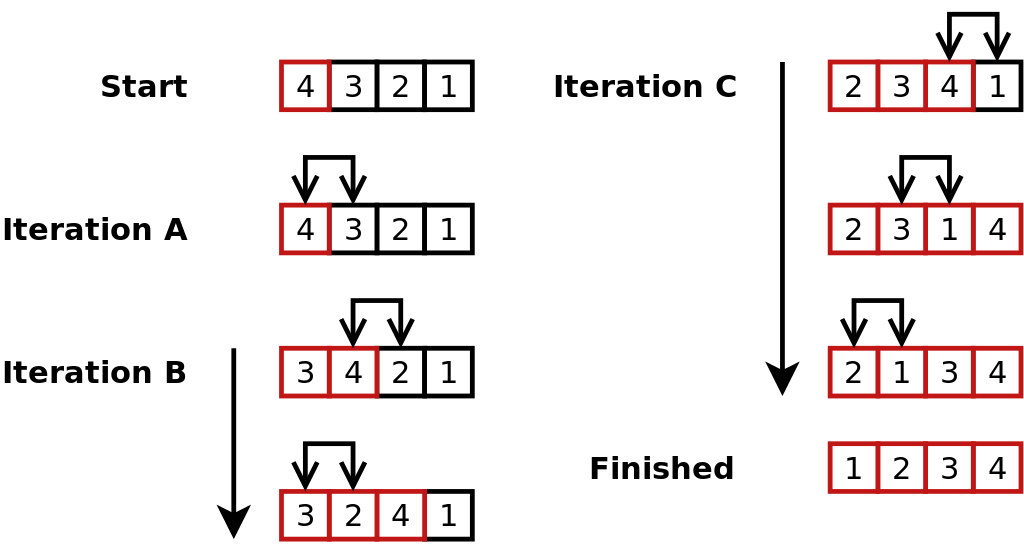
\includegraphics[width=0.8\textwidth]{figures/insertionsort.png}\\
		\hspace*{15pt}\hbox{\scriptsize Image By:\thinspace{\itshape MrDrBob}}
		% https://commons.wikimedia.org/wiki/File:Insertion-sort.svg
	\end{center}
\end{frame}

\begin{frame}
	\frametitle{Insertion Sort}
	\framesubtitle{How does that work?}
		\begin{block}{Insertion Sort}
			The main idea:
			\begin{itemize}
				\item We build the list, step by step.
					\pause
				\item We keep our intermediate result sorted.
					\pause
				\item At every step, we insert the next element into the right place.
					\pause
				\item This means we need to shift over (worst-case) $n$ elements for every element we insert...
					\pause
				\item So in total $\Theta(n^2)$ time.
			\end{itemize}
		\end{block}
\end{frame}

\begin{frame}
	\frametitle{Insertion Sort}
	\begin{algorithmic}
		\State $i \gets 1$ \Comment{The first element forms a sorted list on it's own}
		\pause
		\While{$i < \texttt{len}(l)$}
		\State $j \gets i$
		\pause
		\While{$j > 0$ and $v_{j-1} < v_{j}$}
			\State swap $v_j$ and $v_{j-1}$	
			\State $j \gets j -1$
		\EndWhile
		\pause
		\State $i \gets i+1$
		\EndWhile
	\end{algorithmic}
	\pause
	\begin{center}
	\section{Insertion Sort}
\label{sec:insertion_sort}

\begin{frame}
	\frametitle{Insertion sort}
	\begin{center}
		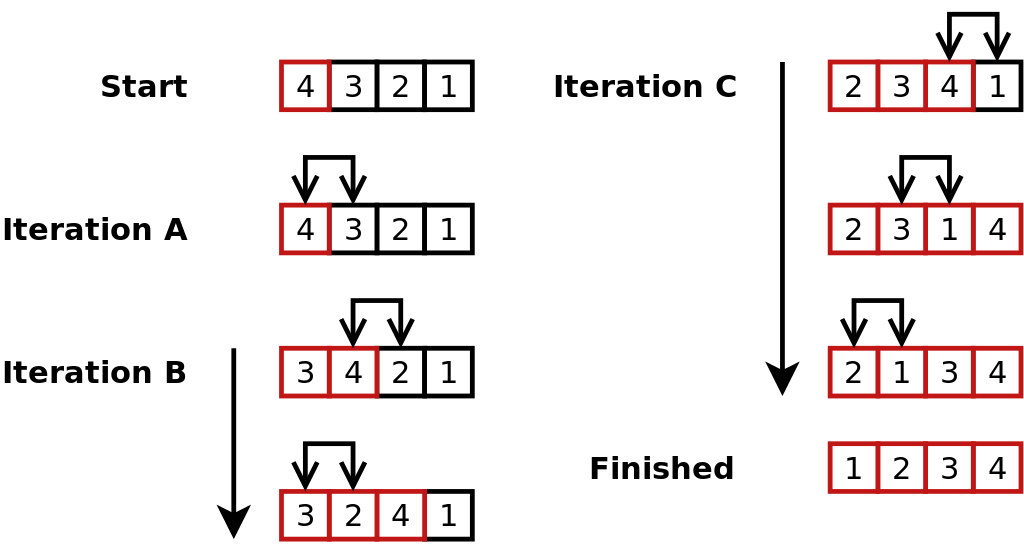
\includegraphics[width=0.8\textwidth]{figures/insertionsort.png}\\
		\hspace*{15pt}\hbox{\scriptsize Image By:\thinspace{\itshape MrDrBob}}
		% https://commons.wikimedia.org/wiki/File:Insertion-sort.svg
	\end{center}
\end{frame}

\begin{frame}
	\frametitle{Insertion Sort}
	\framesubtitle{How does that work?}
		\begin{block}{Insertion Sort}
			The main idea:
			\begin{itemize}
				\item We build the list, step by step.
					\pause
				\item We keep our intermediate result sorted.
					\pause
				\item At every step, we insert the next element into the right place.
					\pause
				\item This means we need to shift over (worst-case) $n$ elements for every element we insert...
					\pause
				\item So in total $\Theta(n^2)$ time.
			\end{itemize}
		\end{block}
\end{frame}

\begin{frame}
	\frametitle{Insertion Sort}
	\begin{algorithmic}
		\State $i \gets 1$ \Comment{The first element forms a sorted list on it's own}
		\pause
		\While{$i < \texttt{len}(l)$}
		\State $j \gets i$
		\pause
		\While{$j > 0$ and $v_{j-1} < v_{j}$}
			\State swap $v_j$ and $v_{j-1}$	
			\State $j \gets j -1$
		\EndWhile
		\pause
		\State $i \gets i+1$
		\EndWhile
	\end{algorithmic}
	\pause
	\begin{center}
	\input{figures/tikz/insertionsort.tex}
	\end{center}
\end{frame}

\begin{frame}
	\frametitle{Would you like some sausages with your cheese?}
	\begin{columns}
		\column{0.455\textwidth}
		\begin{algorithmic}
			\State $i \gets 1$ 
			\While{$i < \texttt{len}(l)$}
			\State $j \gets i$
			\While{$j > 0$ and $v_j < v_{j-1}$}
			\State swap $v_j$ and $v_{j-1}$	
			\State $j \gets j -1$
			\EndWhile
			\State $i \gets i+1$
			\EndWhile
		\end{algorithmic}
		\column{0.455\textwidth}
		\begin{questionblock}{Run time}
			What instance of a list would give the worst performance here?	
		\end{questionblock}
		\pause
		\begin{answerblock}{Again!?}
			Once again it is the reverse list, where every item needs to be moved to the front requiring most swaps.
		\end{answerblock}
		\pause
			\begin{block}{So...}
				The run time is still $\Theta(n^2)$.
			\end{block}	
	\end{columns}

	
\end{frame}

\begin{frame}
	\frametitle{Implementation to summarise}
	
		\begin{alertblock}{See you tomorrow!}
			We will implement this tomorrow :)
		\end{alertblock}	
\end{frame}

\begin{frame}
	\frametitle{Insertion Sort: Pros and Cons}
		\begin{block}{Insertion Sort}
			Repeatedly insert the next item in the correct place in a sorted list.
		\end{block}	
		\begin{exampleblock}{Pros}
			\begin{itemize}
				\item `Easy' algorithm to implement.
				\item Good performance for an $O(n^2)$ algorithm.
			\end{itemize}
		\end{exampleblock}	
		\begin{alertblock}{Cons}
			\begin{itemize}
				\item Still not as fast as comparison-based sorting algorithms can be.
			\end{itemize}
		\end{alertblock}	
	
\end{frame}

	\end{center}
\end{frame}

\begin{frame}
	\frametitle{Would you like some sausages with your cheese?}
	\begin{columns}
		\column{0.455\textwidth}
		\begin{algorithmic}
			\State $i \gets 1$ 
			\While{$i < \texttt{len}(l)$}
			\State $j \gets i$
			\While{$j > 0$ and $v_j < v_{j-1}$}
			\State swap $v_j$ and $v_{j-1}$	
			\State $j \gets j -1$
			\EndWhile
			\State $i \gets i+1$
			\EndWhile
		\end{algorithmic}
		\column{0.455\textwidth}
		\begin{questionblock}{Run time}
			What instance of a list would give the worst performance here?	
		\end{questionblock}
		\pause
		\begin{answerblock}{Again!?}
			Once again it is the reverse list, where every item needs to be moved to the front requiring most swaps.
		\end{answerblock}
		\pause
			\begin{block}{So...}
				The run time is still $\Theta(n^2)$.
			\end{block}	
	\end{columns}

	
\end{frame}

\begin{frame}
	\frametitle{Implementation to summarise}
	
		\begin{alertblock}{See you tomorrow!}
			We will implement this tomorrow :)
		\end{alertblock}	
\end{frame}

\begin{frame}
	\frametitle{Insertion Sort: Pros and Cons}
		\begin{block}{Insertion Sort}
			Repeatedly insert the next item in the correct place in a sorted list.
		\end{block}	
		\begin{exampleblock}{Pros}
			\begin{itemize}
				\item `Easy' algorithm to implement.
				\item Good performance for an $O(n^2)$ algorithm.
			\end{itemize}
		\end{exampleblock}	
		\begin{alertblock}{Cons}
			\begin{itemize}
				\item Still not as fast as comparison-based sorting algorithms can be.
			\end{itemize}
		\end{alertblock}	
	
\end{frame}

	\end{center}
\end{frame}

\begin{frame}
	\frametitle{Would you like some sausages with your cheese?}
	\begin{columns}
		\column{0.455\textwidth}
		\begin{algorithmic}
			\State $i \gets 1$ 
			\While{$i < \texttt{len}(l)$}
			\State $j \gets i$
			\While{$j > 0$ and $v_j < v_{j-1}$}
			\State swap $v_j$ and $v_{j-1}$	
			\State $j \gets j -1$
			\EndWhile
			\State $i \gets i+1$
			\EndWhile
		\end{algorithmic}
		\column{0.455\textwidth}
		\begin{questionblock}{Run time}
			What instance of a list would give the worst performance here?	
		\end{questionblock}
		\pause
		\begin{answerblock}{Again!?}
			Once again it is the reverse list, where every item needs to be moved to the front requiring most swaps.
		\end{answerblock}
		\pause
			\begin{block}{So...}
				The run time is still $\Theta(n^2)$.
			\end{block}	
	\end{columns}

	
\end{frame}

\begin{frame}
	\frametitle{Implementation to summarise}
	
		\begin{alertblock}{See you tomorrow!}
			We will implement this tomorrow :)
		\end{alertblock}	
\end{frame}

\begin{frame}
	\frametitle{Insertion Sort: Pros and Cons}
		\begin{block}{Insertion Sort}
			Repeatedly insert the next item in the correct place in a sorted list.
		\end{block}	
		\begin{exampleblock}{Pros}
			\begin{itemize}
				\item `Easy' algorithm to implement.
				\item Good performance for an $O(n^2)$ algorithm.
			\end{itemize}
		\end{exampleblock}	
		\begin{alertblock}{Cons}
			\begin{itemize}
				\item Still not as fast as comparison-based sorting algorithms can be.
			\end{itemize}
		\end{alertblock}	
	
\end{frame}

	\end{center}
\end{frame}

\begin{frame}
	\frametitle{Would you like some sausages with your cheese?}
	\begin{columns}
		\column{0.455\textwidth}
		\begin{algorithmic}
			\State $i \gets 1$ 
			\While{$i < \texttt{len}(l)$}
			\State $j \gets i$
			\While{$j > 0$ and $v_j < v_{j-1}$}
			\State swap $v_j$ and $v_{j-1}$	
			\State $j \gets j -1$
			\EndWhile
			\State $i \gets i+1$
			\EndWhile
		\end{algorithmic}
		\column{0.455\textwidth}
		\begin{questionblock}{Run time}
			What instance of a list would give the worst performance here?	
		\end{questionblock}
		\pause
		\begin{answerblock}{Again!?}
			Once again it is the reverse list, where every item needs to be moved to the front requiring most swaps.
		\end{answerblock}
		\pause
			\begin{block}{So...}
				The run time is still $\Theta(n^2)$.
			\end{block}	
	\end{columns}

	
\end{frame}

\begin{frame}
	\frametitle{Implementation to summarise}
	
		\begin{alertblock}{See you tomorrow!}
			We will implement this tomorrow :)
		\end{alertblock}	
\end{frame}

\begin{frame}
	\frametitle{Insertion Sort: Pros and Cons}
		\begin{block}{Insertion Sort}
			Repeatedly insert the next item in the correct place in a sorted list.
		\end{block}	
		\begin{exampleblock}{Pros}
			\begin{itemize}
				\item `Easy' algorithm to implement.
				\item Good performance for an $O(n^2)$ algorithm.
			\end{itemize}
		\end{exampleblock}	
		\begin{alertblock}{Cons}
			\begin{itemize}
				\item Still not as fast as comparison-based sorting algorithms can be.
			\end{itemize}
		\end{alertblock}	
	
\end{frame}
